\documentclass[10pt]{article}

\usepackage{answers}
\usepackage{setspace}
\usepackage{graphicx}
\usepackage{enumitem}
\usepackage{multicol}
\usepackage{circuitikz}
\usepackage{adjustbox}
\usepackage{mathrsfs}
\usepackage{mathtools}
\usepackage{svg}
\usepackage[margin=0.5in]{geometry} 
\usepackage{amsmath,amsthm,amssymb}

\newcommand{\N}{\mathbb{N}}
\newcommand{\Z}{\mathbb{Z}}
\newcommand{\C}{\mathbb{C}}
\newcommand{\R}{\mathbb{R}}
\newcommand*{\Co}[2]{{}^{#1}C_{#2}}%

\DeclareMathOperator{\sech}{sech}
\DeclareMathOperator{\csch}{csch}
 
\newenvironment{theorem}[2][Theorem]{\begin{trivlist}
\item[\hskip \labelsep {\bfseries #1}\hskip \labelsep {\bfseries #2.}]}{\end{trivlist}}
\newenvironment{definition}[2][Definition]{\begin{trivlist}
\item[\hskip \labelsep {\bfseries #1}\hskip \labelsep {\bfseries #2.}]}{\end{trivlist}}
\newenvironment{proposition}[2][Proposition]{\begin{trivlist}
\item[\hskip \labelsep {\bfseries #1}\hskip \labelsep {\bfseries #2.}]}{\end{trivlist}}
\newenvironment{lemma}[2][Lemma]{\begin{trivlist}
\item[\hskip \labelsep {\bfseries #1}\hskip \labelsep {\bfseries #2.}]}{\end{trivlist}}
\newenvironment{exercise}[2][Exercise]{\begin{trivlist}
\item[\hskip \labelsep {\bfseries #1}\hskip \labelsep {\bfseries #2.}]}{\end{trivlist}}
\newenvironment{solution}[2][Solution]{\begin{trivlist}
\item[\hskip \labelsep {\bfseries #1}]}{\end{trivlist}}
\newenvironment{problem}[2][Problem]{\begin{trivlist}
\item[\hskip \labelsep {\bfseries #1}\hskip \labelsep {\bfseries #2.}]}{\end{trivlist}}
\newenvironment{question}[2][Question]{\begin{trivlist}
\item[\hskip \labelsep {\bfseries #1}\hskip \labelsep {\bfseries #2.}]}{\end{trivlist}}
\newenvironment{corollary}[2][Corollary]{\begin{trivlist}
\item[\hskip \labelsep {\bfseries #1}\hskip \labelsep {\bfseries #2.}]}{\end{trivlist}}
\pagenumbering{gobble}
\begin{document}
 
% --------------------------------------------------------------
%                         Start here
% -------------------------------------------------------------
\title{Points to Remember}%replace with the appropriate homework number
\author{Aditya Arora} %if necessary, replace with your course title
\maketitle
%Below is an example of the problem environment


\begin{enumerate}
\item \textbf{For Asynchronous circuits:} The outputs are only to be written for the stable state condition while the other input conditions are all outputting don't cares i.e. $X$ or $-$
\item \textbf{Fundamental mode:} The state diagram assuming fundamental mode operation (output is shown as a Moore output but it only assumes that value if the state is stable)
\item \textbf{State Reduction Table:} All states except first vertically down, all states except last horizontally right
% \item \textbf{Karnaugh Map Numbering:} 0 $\rightarrow$ 1 $\rightarrow$ 3 $\rightarrow$ 2 vertically downward in column 1 and the rest will follow easily
\item \textbf{POS and SOP:} SOP $\rightarrow$ 1 and POS $\rightarrow$ 0 (to remember when writing equation from K-Map)
\item \textbf{Asynchronous circuit analysis:} Question 13 from Assignment 10 is so smart, so many little tricks combined
\item \textbf{Writing DFF equation:} The DFF equations can be written directly since the property $Q(t+1) = D$ is valid
\item \textbf{Mealy and Moore:} Mealy output on arrows, Moore output in state
\item \textbf{ASM: }\parbox{\linewidth}{
        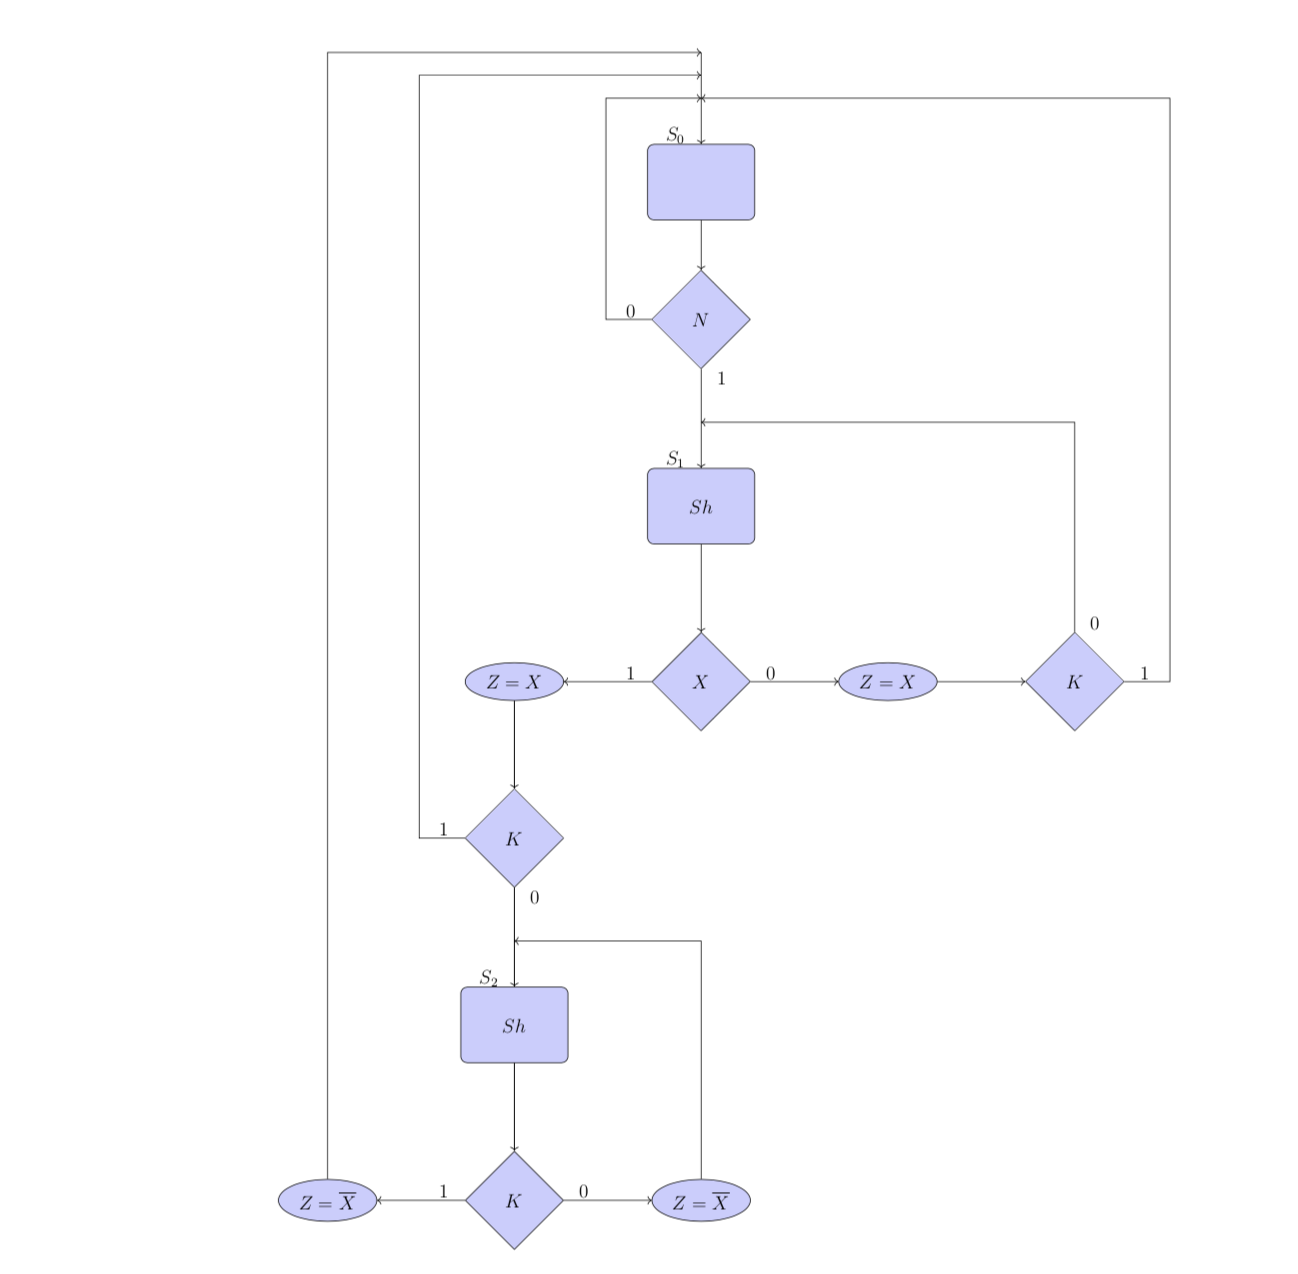
\includegraphics[scale=0.5]{ASM.png}
    }
    \medskip
    See the ``Sh'' shift signal for state dependent outputs\newpage
\item \textbf{4 Bit Bi-Directional shift register using D Flip Flops: }\\
\parbox{\linewidth}{
        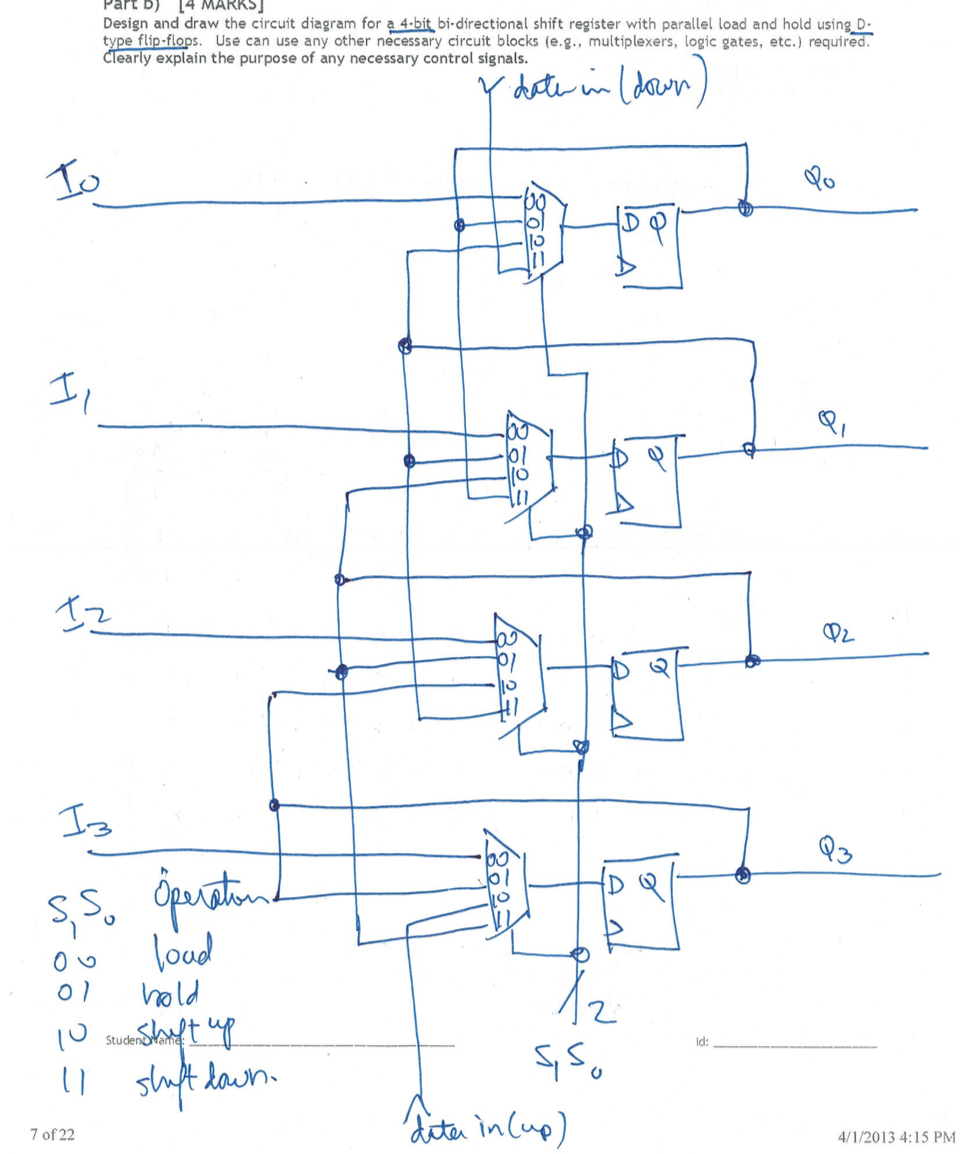
\includegraphics[scale=1]{4BIT.png}
    }
\item \textbf{ASM:} ASM State changes are clocked by the edge
\item \textbf{f:} $T_{clock} + T_{setup} + T_{data} = T \Rightarrow f_{max} = \frac{1}{T}$
\item \textbf{State Machine Diagram to Timing Diagram:} Output follows in Mealy diagram\newpage
\item \textbf{DFF Equations:}\\
\parbox{\linewidth}{
        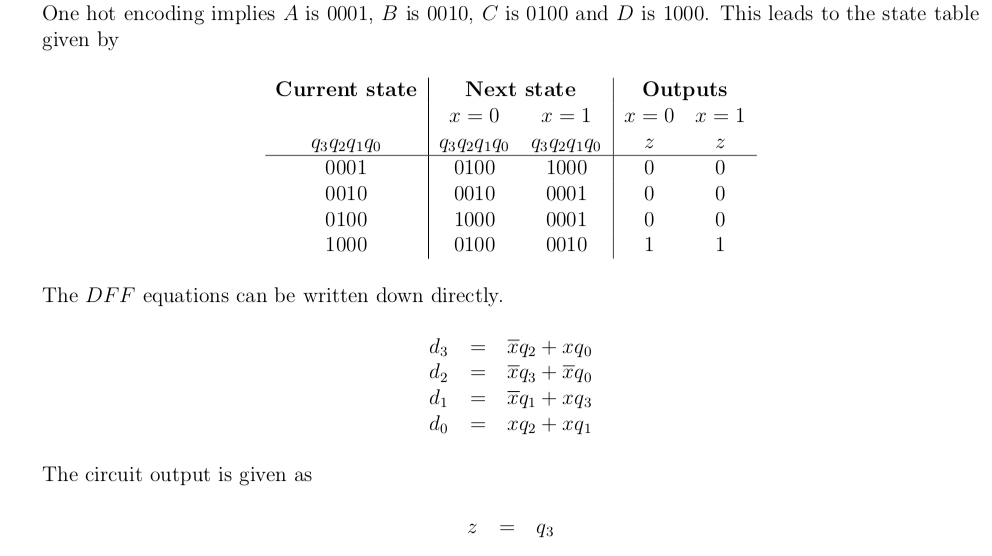
\includegraphics[scale=1]{DFF.png}
    }
\\
\parbox{\linewidth}{
        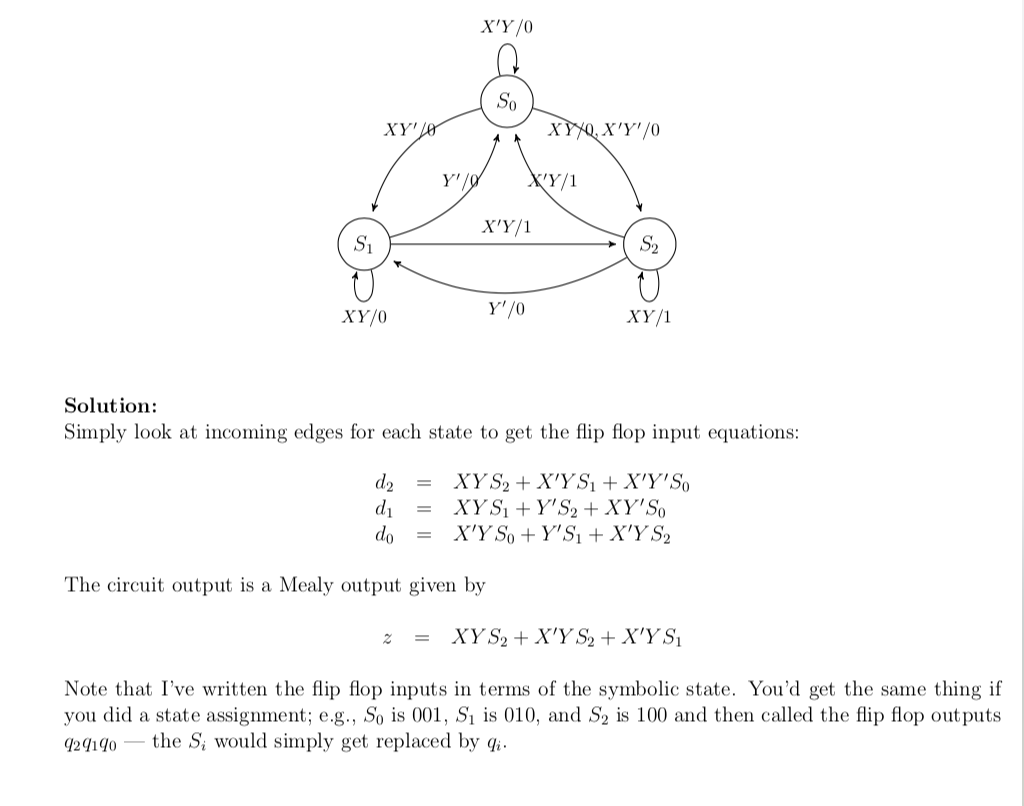
\includegraphics[scale=1]{DFF2.png}
    }
\end{enumerate}



\pagebreak
\setlength{\voffset}{0.15in}

\end{document}
